% Generar PNG
% convert -density 600 fsmexample.pdf -quality 95 fsmexample.png

\documentclass[crop,tikz]{standalone}% 'crop' is the default for v1.0, before it was 'preview'
%\usetikzlibrary{...}% tikz package already loaded by 'tikz' option
\usepackage{tikz}
\usetikzlibrary{automata, positioning, arrows}

\tikzset{
->, % makes the edges directed
%>=stealth’, % makes the arrow heads bold
node distance=3cm, % specifies the minimum distance between two nodes. Change if necessary.
every state/.style={thick, fill=gray!10}, % sets the properties for each ’state’ node
initial text=$ $, % sets the text that appears on the start arrow
}

\begin{document}
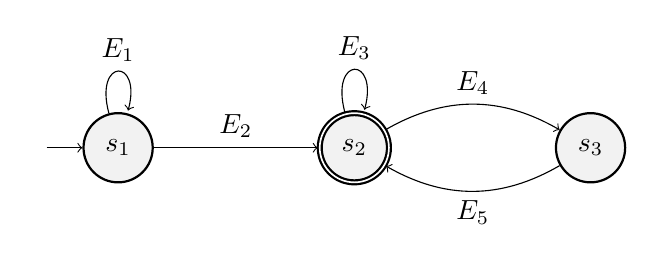
\begin{tikzpicture}
\node[state, initial] (q1) {$s_1$};
\node[state, accepting, right of=q1] (q2) {$s_2$};
\node[state, right of=q2] (q3) {$s_3$};

\draw (q1) edge[loop above] node{$E_1$} (q1)
(q1) edge[above] node{$E_2$} (q2)
(q2) edge[loop above] node{$E_3$} (q2)
(q2) edge[bend left, above] node{$E_4$} (q3)
(q3) edge[bend left, below] node{$E_5$} (q2);
\end{tikzpicture}
\end{document}
